\section{Tuning shared memory code}


\chapterDescription
  {
    Around 30 minutes.
  }
  {
    A working shared memory code.
  }


In this section, we discuss some aspects of shared memory parallelisation and
give some hints for proper shared memory parallelisation.


\subsection{Profiling}

Like any other optimisation, I do recommend to start with some profiling. This
should comprise the usage of proper profilers such as VTune Amplifier, but it
also should comprise at least one run where you
enable Peano's profiling outputs as discussed in
Section \ref{section:performance-analysis}.

Once you have obtained a program output with Peano's performance analysis
enabled, please pass this output to Peano's performance analysis scripts:
\begin{code}
python .../src/peano/performanceanalysis/performanceanalysisroutines.py
\end{code}
\noindent
Invoking the script without any argument displays some usage messages.


\begin{remark}
 Profiling Peano's shared memory behaviour induces a significant runtime
 overhead. Furthermore, it generates lots of code. As a result, Peano does some
 in-situ data accumulation. In return, it means that you have to run the code
 for a decent time and on decent problem sizes to get meaningful results.
 Otherwise, the accumulation does average out too many details.
\end{remark}


\begin{center}
 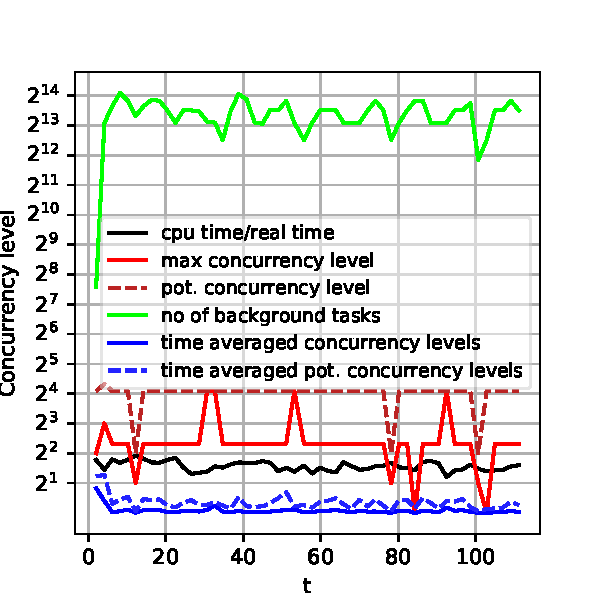
\includegraphics[width=0.6\textwidth]{67_shared-memory-tuning/trace-concurrency.pdf}
\end{center}

\noindent
Peano's shared memory profiling yields four different types of data.
These data stem from very small time sampling intervals. While the data is
sampled in small intervals, Peano dumps the aggregated data to the terminal only
every few seconds. As a result, data is noisy/smoothed out.
The data sets are coloured and we typically distinguish actual concurrency
behaviour to behaviour that could have been obtained if we had split up all
parallel codes into tiny little atomic tasks:

\begin{enumerate}
  \item The ``measured'' concurrency level is the cpu time burnt divided by the
  real time. Usually, this should be around the number of cores/threads you use
  as your system charges you for every physical thread.
  \item The maximum concurrency is the maximum number of threads that could have
  been idle over a small time interval. Peano works in terms of tasks. If the
  number of tasks exceeds the number of threads, the observed concurrency is
  smaller than the derived maximum concurrency. 
  \item The time averaged concurrency weights the individual subsamples averaged
  into one data dump with the underlying time spans, i.e.~it is something alike
  $\frac{\int _T f dt }{|T|}$.
  \item The number of background tasks tries to estimate how many background
  tasks are available at any given time. Peano does not realise a mechanism
  tracking the real number of background tasks, so this is a lower bound. There
  might be more tasks still pending in your system.
\end{enumerate}


\subsection{The measured concurrency level equals two}

\begin{smell}
 The measured concurrency level equals two no matter how many cores we try to
 use. Peano runs on a machine with more than one core.
\end{smell}

\noindent
As all cores today offer hyperthreading, we've ran into this smell when the
operating system/scheduler did mask/pin our code onto exactly one core. 
The code then uses the hyperthread, but cannot really scale beyond the core.
This is for example done by IBM's load balancer if you don't set the OpenMP
threads correctly---even if you don't use OpenMP but TBBs.

 
\subsection{Low concurrency levels}


\begin{smell}
 The (theoretical) concurrency level (black line) is very small. As a result,
 the obtained concurrency level is small, too.
\end{smell}

\noindent
There are multiple ways to tackle such a behaviour. Their ultimate goal is to
increase the concurrency of the code. However, you have to be careful: A
brilliant concurrency does not automatically mean that the code runs faster as
threads might be too small. So any optimisation here deserves a careful tracking
of total runtimes.

\begin{enumerate}
  \item Whenever Peano runs into a set of independent events such as
  \texttt{touchVertexFirstTime}, it does not automatically trigger them in
  parallel. Instead it first computes the cardinality of this set and then asks
  an oracle whether to process this set in parallel. The oracle not only says
  yes/no but also identifies well-suited grain sizes, i.e.~the minimal subset
  size. If you observe a low concurrency, it is a straightforward strategy to
  play around with the settings of the dummy oracle (if you use this one;
  cmp.~Section \ref{section:shared-memory:preparation}) or to use another oracle
  that is able to learn and to adopt the grain sizes automatically. You might also
  decide to write your own oracle.
  \item Whenever Peano runs into a set of (potentially) concurrent events, it
  evaluates the corresponding mapping specifications which concurrency
  constraints have to hold. Basically, they define in a colouring language
  (similar to red-black Gau\ss-Seidel) which events may run in parallel. If an
  adapter merges multiple events, the most restrictive constraint system
  dominates. If your overall concurrency level is too small, it is thus worth to
  study whether these constraint systems can be relaxed.
  \item Finally, you might decide to parallelise your own code within the
  mappings.
\end{enumerate}


\begin{remark}
  The mapping specifications are \textbf{not} static, i.e.~they can evaluate the
  mapping's state. In several projects, I found that some very restrictive
  colouring schemes are mandatory (in classic multigrid, I need often for
  example a $7^d$ colouring to ensure that no two vertices restrict their
  residual at the same time to a coarse vertex). However, they are not mandatory
  all the time, i.e.~I can make the specification query return a less
  restrictive pattern from time to time which speeds up the code significantly.
\end{remark}

\noindent
If you program your own code, you might want to use Peano's
\texttt{peano::grid::datatraversal::} \texttt{TaskSet} to split up your code
into multiple tasks. It then is independent of TBB/OpenMP. Furthermore, there's a macro
\texttt{pfor} in the \texttt{tarch/multicore} directory that allows you to write
parallel for loops that are again independent of the underlying shared memory
parallelisation scheme. A d-dimensional extension exists, too.

All of these helper functions again require a grain size which determines
whether and with which cardinality problems are to be split up.
You can use Peano's oracle mechanism here.
Whenever you ask the oracle for a grain size, you have to pass it the code
location.
Usually such a flag indicates some part of the grid management.
However, there's also a set of user-defined markers.
Use those (you have to bookkeep which ones you use where) to integrate into
Peano's oracle mechanism.

 
Here is an example from the ExaHyPE project where we use the tenth user-defined
marker:
\begin{code}
#include "tarch/multicore/Loop.h"

[...]

const int ProblemSize = ...;
auto grainSize = peano::datatraversal::autotuning::Oracle::getInstance().parallelise(
 ProblemSize,
 peano::datatraversal::autotuning::MethodTrace::UserDefined9
); 
// equals for(int i=0; i<ProblemSize; i++)
pfor(i, 0, ProblemSize, grainSize.getGrainSize())
  [...]
endpfor
grainSize.parallelSectionHasTerminated();
\end{code}



\subsection{Low time-averaged concurrency}

To identify/hunt down this issue, I strongly recommend that you switch off all
of your background tasks, i.e.~tasks you fire and later check for completion.
Tasks running independently in the background are a powerful tool to exploit
many cores, but they also tend to make performance data more difficult to
digest.
Furthermore, they help to exploit the cores but the core grid stuff usually
should already scale all alone without them, i.e.~they cannot compensate for a
poor grid concurrency.


\begin{smell}
  The time averaged concurrency is very small though both the maximum
  concurrency level and the cpu occupation (cpu time by real time) both exceed
  the core count. The code is not really fast.
\end{smell}

\noindent
The plot we are speaking about here are the blue lines. If they are small but
the black line approaches the number of cores, we have to assume that the code
consists of a lot of small tasks that are computationally very cheap.
While the code exploits the cores to process work concurrently, it spends quite
some time in administrating these tasks (scheduling) and running through serial
code parts that are sprinkled in between all the parallel code parts.
Furthermore, it might do quite some data consistency operations.


There is no siler bullet in this case, i.e.~if you can't increase the arithmetic
intensity significantly, you basically have to run through a series of trial and
error ideas without any guarantee of success:

\begin{enumerate}
  \item Peano internally realises a BSP-style data flow: Whenever the grid
  traversal runs into some section of the code that shall run in parallel, it
  copies all the mapping objects and triggers the parallel traversal. Once this
  traversal has terminated, it merges all the mappings again. Obviously, this is
  unneccessary overhead if the mappings' states do not change. In this case, we
  could omit the copying and the merging. To tell Peano to skip them, please set
  the last entry in the corresponding event specifications to \texttt{false}:
  \begin{code}
peano::MappingSpecification  
myprobject::mappings::MyMaping::ascendSpecification(int level) { 
 return peano::MappingSpecification(
  peano::MappingSpecification::Nop,
  peano::MappingSpecification::AvoidCoarseGridRaces,
  false // This false eliminates all the copying 
 );
}
  \end{code}
  In most of my own experiments, manipulating this flag howeve has only a very
  limited impact; often, it even backfires.
  \item Peano internally linearises the whole spacetree and, when it runs
  through the tree, reads on one data stream and pipes out the data stream for
  the subsequent iteration. There is an alternative storage scheme that is
  applies if a whole region of the grid remains stationary, is regular and the
  shared memory parallelisation tells the code to do so\footnote{The  design
  here is slightly flawed---a decision which storage format to choose has
  basically nothing to do with shared memory parallelisation. We hijack the
  shared memory decision making nevertheless as this storage decision starts to
  have its major influence once shared memory parallelisation is switched on.}.
  If you have a rather regular, starionary grid, you can doublecheck which
  storage format is chosen by letting \texttt{peano::grid} plot its stuff. You
  should obtain messages alike
  \begin{code}
  regular grid of height 5 used nonpersistently/persistently=0/1 times
  \end{code}
  and the index left of the \texttt{/} should be high(er). It depends on the
  type of shared memory oracle whether you can manually enforce a persistent
  storage. Please study the constructor's arguments.
\end{enumerate}


\begin{center}
 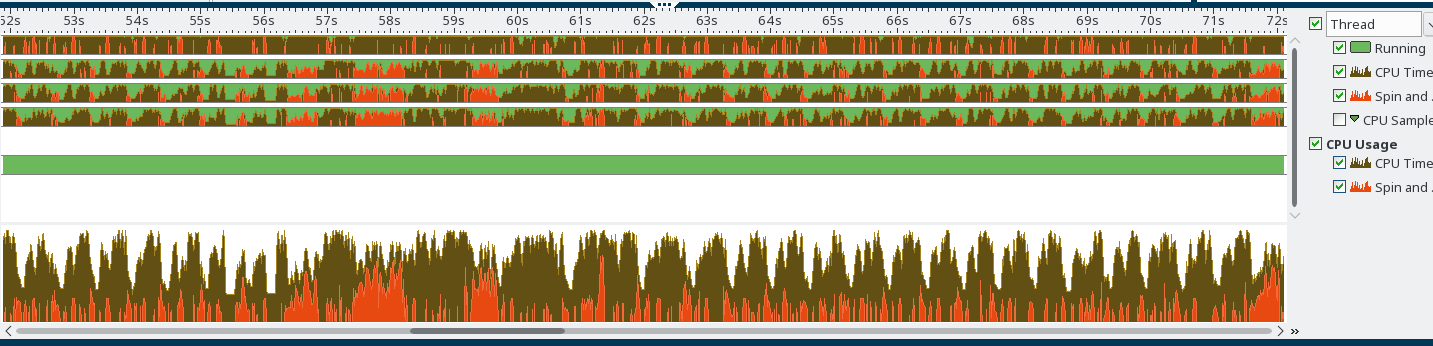
\includegraphics[width=0.8\textwidth]{67_shared-memory-tuning/vtune.png}
 \\
 {\footnotesize
  Typically VTune snapshot that uncovers very high spinning timings.  
 }
\end{center}

\begin{smell}
  The time averaged concurrency is very small though the code seems to exploit
  all cores. VTune complains about a lot of spinning.
\end{smell}

\noindent
There are basically two things you can do: 

\begin{enumerate}
  \item You can increase the grain sizes delivered by the shared memory oracles.
  If you use autotuning, this should automatically be done.
  \item If you use background tasks, try to fuse multiple of these tasks into
  a single one.
\end{enumerate}


\begin{center}
 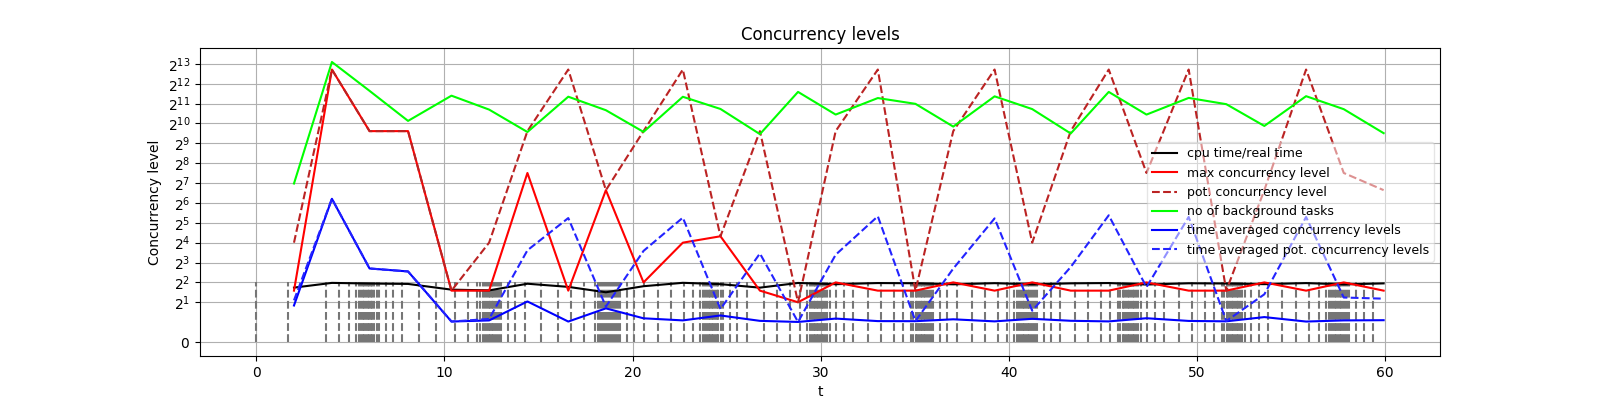
\includegraphics[width=0.8\textwidth]{67_shared-memory-tuning/concurrency.png}
 \\
 {\footnotesize
  Profile obtained through Peano's built-in profiling on a two-core laptop that
  shows that many background tasks would be available if there were more cores.
 }
\end{center}
